% CLASE
\documentclass[a4paper,12pt]{article}

% PREÁMBULO
% Paquetes:
\usepackage[spanish]{babel}
\usepackage{graphicx}
\usepackage{tikz,color}
\usepackage{pgf-pie}
\usepackage{pgfgantt}
\usepackage{pdflscape}
\usepackage[backend=biber]{biblatex}
\bibliography{Recursos/Bibliografia}

% CUERPO
\begin{document}

% Caratula
    \begin{titlepage}
        \centering
        
\includegraphics[width=0.2\textwidth]{Imagenes/LogoUTN.png}\par
        \vfill
        {\bfseries\LARGE Universidad Tecnológica Nacional \par}
        \vfill
        {\scshape\Large Facultad Regional Rosario \par}
        \vfill
        {\scshape\Huge Aplicación de Apoyo al Cuidado de Personas \par}
        \vfill
        {\itshape\Large Ingeniería en Sistemas de Información \par}
        {\itshape\Large Proyecto Final de Carrera \par}
        \vfill
        {\Large Autores: \par}
        {\Large Carignani, Esteban Agustín \par}
        {\Large Culich, María Agustina \par}
        {\Large Montisori, Agustín \par}
        \vfill
        {\Large Tutor: \par}
        {\Large Stortoni, Silvia \par}
        \vfill
        {\Large Abril 2024 \par}
    \end{titlepage}

% Abstract
    \begin{abstract}
        Cuidar de otra persona, ya sea un adulto mayor, 
        un niño, una persona con discapacidad o alguien 
        con una enfermedad, puede ser una tarea compleja. 
        La gestión de medicamentos, horarios, cuidadores, 
        turnos, recordatorios médicos y la comunicación 
        entre las personas involucradas.
        Basándonos en las respuestas de una encuesta realizada enfocada a personas que tienen a su cargo el cuidado de otras, presentamos una aplicación móvil innovadora que facilita la gestión y organización de las tareas que implica estar al cuidado de alguien más. Nuestra propuesta es una app que permitiría el registro de información personal de la persona bajo cuidado y la asociación de esta al cuidador, centralización de la comunicación entre ambas partes y terceros involucrados, simplicidad en la organización de visitas y turnos médicos, agenda de medicación, tareas cotidianas, etc. Además, se incluirán herramientas que respondan a las necesidades relevadas en el cuestionario de sondeo.
    \end{abstract}

    \newpage

% Tabla de contenidos
    \tableofcontents 
    
    \newpage

% Análisis de la organización
    \section{Analisis de la organización}
    Partiendo de la base en que para el proyecto no existe una organización u empresa definida particular en la cuál apoyarnos, el análisis organizacional que llevaremos a cabo pone foco principal en el equipo de desarrollo del proyecto en cuestión, considerando al mismo como una \textit{startup} que se inicia en el mercado de desarrollo de soluciones informáticas. Concentrando los esfuerzos principalmente en las capacidades y recursos del equipo a cargo.\newline
    El objetivo es evaluar la estructura del equipo, habilidades, procesos de trabajo, disponibilidad de recursos financieros y tecnológicos, definición de fortalezas, debilidades y oportunidades que pueden afectar al desarrollo del equipo como organización.
    \subsection{BubiSoft}
    La empresa toma como punto de partida inicial el desarrollo de soluciones informáticas orientadas a problemáticas sociales y cotidianas de las personas.\newline
    El mercado al que apunta la organización y sobre el cual sienta las bases de su crecimiento es el siguiente:
    \begin{itemize}
        \item Sujetos que se enfrentan ante una situación específica que deriva en la necesidad de tener una o más personas encargadas.
        \item Familiares o red de contención que se encargan del cuidado de una o más personas dependientes o parcialmente dependientes y de todas las tareas que engloba.
    \end{itemize}
    Tomando esto en consideración, procedemos a la realización del análisis que nos permite determinar la misión, visión y objetivos de la organización.
    \subsection{Misión}
    Brindar soluciones tecnológicas que simplifiquen la atención a las problemáticas cotidianas para aquellas personas que se encuentren en situación de vulnerabilidad y sirvan de apoyo para con los responsables del cuidado.
    \subsection{Visión}
    Posicionarse como una de las principales consultoras tecnológicas responsables de brindar soluciones informáticas innovadoras para abordar diversas problemáticas sociales.
    \subsection{Objetivos principales}
    \begin{itemize}
        \item Brindar soluciones tecnológicas que mejoren la calidad de vida de las personas mayores y faciliten la labor de sus cuidadores.
        \item Alcanzar la sostenibilidad financiera y un crecimiento rentable a largo plazo, posicionándose de forma estratégica en el mercado de soluciones informáticas.
        \item Contribuir a mejorar el bienestar general de la sociedad, estudiando y evaluando con atención sus necesidades y contribuyendo con formas de satisfacerlas a través del desarrollo de nuevas tecnologías.
    \end{itemize}
    \subsection{Objetivos secundarios}
    \begin{enumerate}
        \item \underline{Organizacionales}
        \begin{itemize}
            \item Identificar las necesidades específicas de las personas.
            \item Desarrollar soluciones tecnológicas fáciles de usar e intuitivas para los usuarios.
            \item Ofrecer funcionalidades que aborden las necesidades más comunes.
            \item Desarrollar un sólido modelo de negocio que genere ingresos a través de suscripciones.
            \item Atraer y retener usuarios.
            \item Explorar oportunidades de expansión en mercados similares.
        \end{itemize}
        \item \underline{Sociales}
        \begin{itemize}
            \item Reducir la carga de trabajo de los cuidadores y familiares.
            \item Promover la independencia y autonomía de las personas mayores.
            \item Reducir los niveles de aislamiento social y soledad de las personas mayores.
            \item Concientizar a la sociedad sobre los desafíos que representan la etapa de envejecimiento.            
        \end{itemize}
    \end{enumerate}
    \subsection{Organigrama}
    Si bien la empresa resulta ser una startup inicial que consta de pocas personas integrándola, realizamos el organigrama basándonos en los roles y funciones que cumplen sus integrantes.\newline
    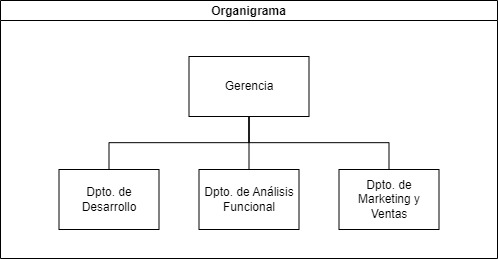
\includegraphics[width=1\textwidth]{Imagenes/Organigrama.jpg}\newline
    Profundizaremos un poco más en las tareas a cargo de cada uno de los departamentos que integran a la empresa.
    \begin{itemize}
        \item[\textbf{Gerencia:}] Se compone del equipo fundador de la empresa, encargados de la toma de decisiones relacionadas al futuro de la empresa, el camino a seguir y los proyectos a encarar.
        \item[\textbf{Desarrollo:}] Es el departamento a cargo del arquitecto de software, quien coordina a todos los desarrolladores a lo largo de la codificación, desarrollo y mantenimiento del software.
        \item[\textbf{Análisis:}] Este departamento está a cargo del líder de proyectos, a su mando están los analistas y testers, encargados de relevar, comprender e interpretar las necesidades de los clientes y asegurar que las mismas se satisfagan correctamente por el software implementado.
        \item[\textbf{Marketing:}] El departamento de marketing se encarga de publicitar, publicar y promover el uso de la aplicación desarrollada. A su vez, sus tareas incliuyen realizar campañas de retención de usuarios, escuchando las críticas que estos ofrezcan, y comunicándolas al departamento de análisis. 
    \end{itemize}
    \subsection{Matriz FODA}
    \textbf{\underline{Fortalezas}}
    \begin{itemize}
        \item[] \textit{Enfoque en problemática social:} Al centrarse en atender una necesidad real y creciente de la sociedad, la empresa da un propósito claro, apuntado a un mercado real de potenciales clientes.
        \item[] \textit{Soluciones innovadoras:} La empresa propone soluciones tecnológicas novedosas y adaptadas a las necesidades específicas de las personas.
        \item[] \textit{Potencial de impacto:} Las soluciones tienen el potencial de mejorar significativamente la calidad de vida de las personas, generando un impacto positivo en la sociedad.
        \item[] \textit{Alta motivación:} Al ser una empresa que está en sus inicios, sus integrantes están altamente motivados para enfrentar los diferentes desafíos de forma proactiva e inmediata.
    \end{itemize}
    \textbf{\underline{Oportunidades}}
    \begin{itemize}
        \item[] \textit{Innovación:} Los nuevos avances en tecnología como la inteligencia artificial y la domótica pueden abrir nuevas posibilidades para el desarrollo de soluciones innovadoras.
        \item[] \textit{Creciente mercado:} De la mano con la revolución tecnológica y el amplio rango de edad que abarcan actualmente las tecnologías, genera una demanda cada vez mayor de soluciones que puedan hacer frente a las necesidades de las personas.
        \item[] \textit{Alianzas estratégicas:} La organización es capaz de asociarse con otras empresas, organizaciones o instituciones enfocadas en temáticas inherentes a las soluciones brindadas, para ampliar su alcance y potenciar su impacto.
    \end{itemize}
    \textbf{\underline{Debilidades}}
    \begin{itemize}
        \item[] \textit{Inexperiencia:} Al ser una startup reciente que incursiona en el desarrollo de soluciones tecnológicas, se enfrenta a los problemas de falta de experiencia a la hora de afrontar desafíos técnicos, financieros y de gestión.
        \item[] \textit{Capital limitado:} Cada decisión a tomar implica un potencial riesgo en la continuidad y estabilidad de la empresa debido al poco capital inicial con el que cuentan.
        \item[] \textit{Escasez de recursos:} El escaso nivel de personal inicial representa una limitante a la hora de tomar posibles proyectos debido al riesgo de caer en una sobrecarga laboral que afecte a las entregas y el éxito de los mismos.
    \end{itemize}
    \newpage
    \textbf{\underline{Amenazas}}
    \begin{itemize}
        \item[] \textit{Avances tecnológicos:} La aparición de nuevas tecnologías pueden crear soluciones a las mismas problemáticas de los proyectos realizados por la empresa pudiendo dejarlos obsoletos.
        \item[] \textit{Dificultades para obtener financiación:} sin el apoyo de programas gubernamentales y organizaciones sin fines de lucro, podría limitar la capacidad de la organización para crear nuevas soluciones.
        \item[] \textit{Mercado competitivo:} El gran nivel de demanda y competencia salarial que presenta el actual mercado de tecnología, dificulta el ingreso competitivo y la rentabilidad inmediata de la empresa.
    \end{itemize}
    \subsection{Procesos principales}
    Tomando en consideración el análisis hecho de la organización, y el foco que hacen en las problemáticas sociales, consideramos los siguientes procesos principales.\newline
    \newline
    \textbf{\underline{Investigación y desarrollo}}\newline
    Dentro de los procesos de investigación y desarrollo incluimos procesos más atómicos cómo:
    \begin{itemize}
        \item[] \textit{Identificación de necesidades:} este proceso engloba la realización de un análisis de las necesidades específicas de los stakeholders tanto a nivel individual cómo a nivel colectivo. Dentro del mismo se engloban tareas cómo la realización de encuestas, entrevistas, grupos focales, etc., que permitan comprender los desafíos y oportunidades que enfrentan.
        \item[] \textit{Diseño y modelado de soluciones:} consiste en diseñar las posibles soluciones tecnológicas innovadoras que hagan frente a las necesidades identificadas previamente, priorizando la facilidad de uso y las capacidades de los usuarios a los que apunta. Se emplean metodologías de modelado centradas en la experiencia de usuario para asegurar la conformidad y usabilidad de las aplicaciones.
        \item[] \textit{Desarrollo de software:} este proceso engloba todas las tareas relacionadas a la materialización de las propuestas tecnológicas planteadas y diseñadas previamente. Se definen y emplean metodologías de desarrollo acordes a las necesidades de cada proyecto y herramientas modernas, asegurando la calidad, seguridad y confiabilidad de las soluciones. Además se incluyen las tareas relacionadas al testing y pruebas para garantizar que las soluciones funcionen correctamente y cumplan con los requisitos establecidos.
    \end{itemize}
    \textbf{\underline{Implementación y soporte}}
    \newline
    Este proceso engloba la salida y puesta en producción de las aplicaciones desarrolladas, junto con el seguimiento y mejora continua de las mismas, atendiendo a las necesidades de los usuarios y las opiniones recibidas.
    \begin{itemize}
        \item[] \textit{Implementación:} engloba el lanzamiento y puesta en producción de las soluciones tecnológicas en los entornos donde se utilizarán, brindando capacitación y asistencia a los usuarios para garantizar una adopción exitosa. Además se pautan mecanismos de seguimiento y evaluación para medir el impacto de las soluciones y realizar mejoras continuas.
        \item[] \textit{Soporte técnico:} consiste en brindar soporte técnico a los usuarios, resolviendo problemas de manera oportuna y eficiente. Para su efectividad, se utilizan canales de comunicación efectivos previamente definidos cómo información de contacto, opiniones y valoración en plataformas de descargas, etc.
        \item[] \textit{Actualizaciones y mantenimiento:} abarca las tareas enfocadas en actualizaciones periódicas de las soluciones tecnológicas para incorporar nuevas funcionalidades, corregir errores y mejorar el rendimiento.
    \end{itemize}
    \textbf{\underline{Gestión y administración}}
    \newline
    Los procesos de gestión y administración son aquellos que alinean los objetivos estratégicos de la empresa con la visión y misión de las mismas, a fin de orientar los esfuerzos colectivos hacia una misma meta.
    \begin{itemize}
        \item[] \textit{Planificación estratégica:} consiste en establecer un plan estratégico que defina los objetivos a largo plazo de la startup, las estrategias para alcanzarlos y los recursos necesarios. Se realizan revisiones periódicas del plan para adaptarlo a las condiciones cambiantes del mercado y las necesidades de los usuarios.
        \item[] \textit{Gestión financiera:} engloba la gestión de los recursos financieros de manera eficiente, asegurando la sostenibilidad de la startup a largo plazo. Realizando periódicamente presupuestos, control de gastos y análisis de rentabilidad que sirvan de apoyo a la hora de tomar decisiones financieras.
        \item[] \textit{Gestión del talento humano:} abarca las tareas relacionadas al reclutamiento, evaluación, selección y capacitación de personal que formará parte de la empresa.
    \end{itemize}
    \textbf{\underline{Marketing y ventas}}
    \newline
    Este proceso engloba todas aquellas tareas relacionadas a la divulgación, promoción y alcance de las soluciones tecnológicas puestas en el mercado. A su vez, engloba la definición de estrategias y planes para potenciar el alcance de la marca y su posicionamiento estratégico en el mercado.
    \begin{itemize}
        \item[] \textit{Estrategia de marketing:} se establece una estrategia publicitaria que permita dar a conocer las soluciones tecnológicas a los usuarios potenciales y generar interés en su adopción. Los principales canales de difusión consisten en la publicidad digital y la valoración en plataformas de descargas.
        \item[] \textit{Ventas:} consiste en la definición de un proceso de ventas efectivo que permita convertir a los clientes potenciales en usuarios reales. Incluye demostraciones de casos de éxito, pruebas gratuitas y planes de suscripción.
        \item[] \textit{Atención al cliente:} abarca los servicios de atención al cliente para fidelizar a los usuarios y resolver sus inquietudes.
    \end{itemize}
    \textbf{\underline{Evaluación y mejora continua}}
    \newline
    Este proceso consiste en monitorear el impacto de las soluciones tecnológicas en la calidad de vida de las personas alcanzadas, utilizando indicadores clave de rendimiento (KPIs) para medir el éxito de las soluciones e identificar áreas de mejora.\newline
    Además, se implementa un proceso de mejora continua capaz de optimizar las soluciones tecnológicas, los procesos internos y las estrategias de negocio, haciendo uso y beneficio de la retroalimentación de los usuarios y los datos recopilados.

    \newpage

% Analisis de problemas
    \section{Análisis de problemas}
    El surgimiento de la iniciativa de realizar un software que se encargue de la gestión y organización de las tareas que implica estar al cuidado de otras personas, se origina en las complejas problemáticas con las que nos encontramos diariamente.\newline
    A fin de poder abordarlas con mayor exactitud y precisión, llevamos a cabo la realización de un cuestionario presentado a unas cincuenta personas, de diferentes edades, oficios y calidades de vida, con preguntas orientadas a sus experiencias en el cuidado de adultos mayores, niños pequeños, personas con alguna condición específica, etc. A partir del mismo, analizamos los resultados y concluimos en las diferentes problemáticas comunes.\newline
    \newline
    \subsection{Gráficas de respuestas}
    En esta sección presentamos las diferentes gráficas correspondientes a cada una de las preguntas realizadas en el relevamiento, que permiten posteriormente identificar potenciales usuarios, problemáticas, funcionalidades, etc.\newline
    El relevamiento fue orientado a aquellas personas que se encuentran en posición de cuidador, ya sea profesionalmente o por algun vínculo en especial.
    \subsubsection{¿Qué vínculo o relación tienen?}
        \begin{tikzpicture}
            \pie[explode={0.2, 0.2, 0.2, 0.2, 0.2, 0.2, 0.2}]
            {35/Familiar, 
            26/Hijos, 
            14/Cuidador, 
            7/Docente, 
            7/Padres, 
            7/Niñeros, 
            4/Hermanos}
        \end{tikzpicture}
    \subsubsection{¿Cuáles son las principales problemáticas que enfrentan?}
        \begin{tikzpicture}
            \pie[explode={0.2, 0.2, 0.2, 0.2, 0.2, 0.2, 0.2, 0.2, 0.2}]
            {30/Cansancio y disponibilidad, 
            14/Comunicación, 
            14/Desconocimiento, 
            12/Organización, 
            12/Responsabilidad, 
            7/No responde, 
            5/Daños y enfermedades, 
            4/Movilidad y entorno, 
            2/Cuidadores}
        \end{tikzpicture}
    \subsubsection{¿Cuáles son las principales formas de comunicación?}
        \begin{tikzpicture}
            \pie[explode={0.2, 0.2, 0.2, 0.2, 0.2}]
            {37/Verbal, 
            17/Escrito informal, 
            16/No responde, 
            16/Whatsapp, 
            14/Escrito formal}
        \end{tikzpicture}
    \subsubsection{¿Cuéntan con ayuda profesional para el cuidado?}
        \begin{tikzpicture}
            \pie[explode={0.2, 0.2, 0.2}, rotate=270]
            {58/Si, 
            32/No, 
            10/No responde}
        \end{tikzpicture}
    \subsubsection{¿Qué funcionalidades crees que te resultarían útiles en la aplicación?}
        \begin{tikzpicture}
            \pie[explode={0.2, 0.2, 0.2}, rotate=290]
            {40/Sin responder,
            14/Información y recursos,
            12/Monitoreo y seguimiento,
            11/Organización del cuidado,
            9/Gestión de emergencias,
            9/Gestión de medicación,
            5/Comunicación y apoyo}
        \end{tikzpicture}
    \subsection{Complejidad en la gestión de tareas de cuidado}
    Cuidar a otra persona implica realizar y controlar una gran variedad de tareas complejas, incluyendo:
    \begin{itemize}
        \item Medicamentos
        \item Horarios
        \item Cuidadores
        \item Turnos médicos
        \item Recordatorios médicos
        \item Comunicación entre las partes involucradas
    \end{itemize}
    \subsection{Falta de organización y centralización de información}
    La información relevante sobre la persona que se encuentra bajo el cuidado de otras personas y las tareas pendientes se encuentra dispersa, lo que dificulta su seguimiento, genera confusión, olvidos y gestión eficiente.
    \subsection{Dificultad en la comunicación y coordinación entre cuidadores}
    La comunicación entre el o los cuidadores principales y otros cuidadores puede ser fragmentada e ineficiente, lo que puede generar confusiones y retrasos.
    \subsection{Falta de herramientas para la gestión de actividades y turnos médicos}
    No existe una herramienta centralizada para organizar y gestionar las actividades, terapias y turnos médicos de la persona bajo cuidado, lo que puede llevar a olvidos y errores.
    \subsection{Ausencia de un sistema de recordatorios para la medicación}
    La falta de un sistema de recordatorios para la medicación puede aumentar el riesgo de errores en la administración de los medicamentos, con potenciales consecuencias negativas para la salud de la persona bajo cuidado.
    \subsection{Necesidades específicas no cubiertas por las soluciones existentes}
    Actualmente en el mercado no existe una herramienta que cuente con las funcionalidades necesarias para solucionar y gestionar todas los requerimientos que implican las problemáticas mencionadas arriba. 

    \newpage

% Analisis de Objetivos
    \section{Análisis de objetivos}
    Teniendo en cuenta las problemáticas identificadas, buscamos encontrar respuestas a ellas planteando una variedad de diferentes objetivos que permitan abordar una solución integral y completa.
    \subsection{Optimizar la gestión de tareas}
    \begin{itemize}
        \item Reducir el tiempo dedicado a tareas administrativas y repetitivas.
        \item Centralizar la información y documentación relevante en un solo lugar.
        \item Automatizar recordatorios y notificaciones para medicamentos, citas y otras tareas.
    \end{itemize}
    \subsection{Mejorar la comunicación y coordinación}
    \begin{itemize}
        \item Facilitar la comunicación fluida entre el o los cuidadores principales y otros cuidadores involucrados.
        \item Crear un espacio para compartir información, actualizaciones y mensajes importantes.
        \item Permitir la coordinación de turnos, visitas y tareas entre cuidadores.
        \item Brindar herramientas para alertar o solicitar asistencia en situaciones de riesgo.
    \end{itemize}
    \subsection{Brindar herramientas para la gestión de la salud}
    \begin{itemize}
        \item Ofrecer una agenda de medicación con sistema de notificaciones y alertas.
        \item Permitir el registro y seguimiento de signos vitales y otros indicadores de salud.
        \item Facilitar el acceso a información sobre enfermedades, tratamientos, procedimientos y recursos de salud.
    \end{itemize}
    \subsection{Atender las necesidades específicas de cada caso}
    \begin{itemize}
        \item Incorporar funcionalidades específicas para diferentes tipos de cuidados, como cuidado de adultos mayores, niños con necesidades especiales, personas con discapacidades o personas con enfermedades crónicas.
        \item Permitir la personalización de la aplicación según las necesidades y preferencias del usuario.
    \end{itemize}
    \subsection{Promover el bienestar del cuidador}
    \begin{itemize}
        \item Reducir el estrés y la carga de trabajo del cuidador.
        \item Facilitar el acceso a recursos de apoyo y asesoramiento.
    \end{itemize}

    \newpage
    
% Alternativas de Solución
    \section{Alternativas de solución}
    Actualmente en el mercado, no existe una aplicación que abarque de forma integral el cuidado de personas dependientes, ya sean adultos mayores, niños pequeños, o aquellos con condiciones particulares que requieran de atención y cuidado constante.\newline
    Las propuestas alternativas existentes en el mercado abarcan algunas de las problemáticas de forma independiente, pero no engloban la totalidad que ofrece nuestra aplicación.\newline
    Nuestra iniciativa de solución surgió a partir de la necesidad real de nuestras propias experiencias, de conocidos y allegados que se encuentran estando a cargo de otras personas, en nuestra experiencia y la de ellos, se utilizan distintas herramientas para ayudar en algunas de las problemáticas, pero ninguna ofrece una solución que las englobe en su totalidad.\newline
    Entre las que encontramos e investigamos, destacamos dos que consideramos próximas al alcance del proyecto en cuestión.
    \subsection{Cuidarlos}
    Cuidarlos es una aplicación que facilita conectar aquellas personas con vocación de servicio en cuidar adultos mayores con aquellos que necesitan los cuidados.
    \subsubsection{Abstract}
    Nuestra misión es generar un ecosistema que garantice acceder al mejor cuidado de las personas, que brinde oportunidades a quienes tienen vocación de servicio para destacarse y que seamos un medio para gestionar simple y eficientemente que la vida independiente en los hogares sea una realidad que mejore significativamente la calidad de quienes sean parte. \newline
    Queremos que todos los que integramos Cuidarlos, los que se sumen como familiares, cuidadores, proveedores, financiadores dejen una verdadera huella positiva en el otro. Que las familias puedan sentir que quienes cuidan de sus seres queridos lo hacen con el mismo cariño, compromiso y respeto como si lo hicieran ellos. Que pueden estar tranquilos que las elecciones que hacen mejoran significativamente la calidad de vida de su ser querido. Deseamos que los cuidadores puedan desarrollarse y estén lo suficientemente formados académica y espiritualmente para dar lo mejor de sí en pos del bienestar de quienes cuidan y sus familias. Que sientan que haber estado en esa etapa de la vida fue significativo y que son parte de muchas familias que les agradecen y valoran contar con ellos. \newline
    Nosotros desde Cuidarlos queremos ser solamente el vehículo que desarrolle este ecosistema, permitiendo dejar esa huella tan significativa que implica cuidar del otro dando lo mejor de nosotros mismos.\cite{Cuidarlos}
    \subsubsection{Funcionalidades}
    Las funcionalidades en común entre ambas aplicaciones son las siguientes:
    \begin{itemize}
        \item Permite conectar con personas dedicadas al cuidado de adultos mayores.
        \item Permite visualizar valoraciones y experiencias de los cuidadores.
        \item Calendario con horarios de ingresos y salidas del cuidador y turnos rotativos.
    \end{itemize}
    Las funcionalidades que no encontramos dentro de la app \textit{Cuidarlos} y si en nuestra propuesta son:
    \begin{itemize}
        \item Permite el chat de comunicación entre las diferentes personas encargadas del cuidado.
        \item Permite recordatorios y registro de medicamentos, signos vitales, estado de ánimo.
        \item Permite la participación entre familiares cómo cuidadores.
        \item Funciones de contacto de emergencia y solicitud de ayuda.
    \end{itemize}
    \subsubsection{Conclusión}
    En conclusión, la aplicación \textit{Cuidarlos} facilita conectar aquellas personas que se dedican al cuidado de los adultos mayores, con quienes necesitan del servicio para sus familiares avanzados de edad. Permite un seguimiento, evaluación y coordinación entre los cuidadores y el adulto mayor, pero excluye de la participación a la persona al cuidado en cuestión. Desde nuestra aplicación, fomentamos e incluimos la participación del mismo, siendo un usuario más de la misma y atendiendo sus necesidades específicas.
    \subsection{MyTherapy}
    Esta aplicación, aborda la problemática desde el enfoque de la salud, permitiendo añadir y registrar recordatorios de pastillas y medicamentos, seguimiento del estado de salud de los adultos mayores en el día a día, reporte e informes del mismo para utilizar cómo respaldo en citas médicas, y conectividad con familiares para que los mismos puedan estar al pendiente de la situación.
    \subsubsection{Abstract}
    Sabemos que llevar al día su medicación y cumplir con sus metas diarias es más fácil decirlo que hacerlo. En MyTherapy nos esforzamos por hacer su vida más fácil. Nuestra misión es simplificar su tratamiento sin importar lo complejo que sea y hacer posible que usted tenga el control de su salud. Somos un equipo internacional formado por diseñadores, desarrolladores y entusiastas de la salud digital, y todos compartimos el mismo objetivo, ayudarle de la mejor manera posible. \cite{MyTherapy}
    \subsubsection{Funcionalidades}
    Dentro de las funciones compartidas por ambas aplicaciones tenemos:
    \begin{itemize}
        \item Recordatorio de medicamentos.
        \item Seguimiento del estado de salud y parámetros de medida.
        \item Informe del estado de salud compartido con familiares.
        \item Conexión con familiares.
    \end{itemize}
    En cuanto a las diferentes funcionalidades que \textit{MyTherapy} no tiene en cuenta en comparación con nuestra propuesta, destacamos:
    \begin{itemize}
        \item Calendario de actividades relacionadas al cuidado de la salud de la persona.
        \item Registro de cuidadores o familiares responsables del cuidado.
        \item Participación activa de los familiares en el cuidado de las personas.
        \item Comunicación entre los diferentes cuidadores responsables.        
    \end{itemize}
    \subsubsection{Conclusión}
    En conclusión, \textit{MyTherapy} aborda de una manera completa la problemática relacionada con los recordatorios del plan de salud del adulto mayor. Pero no incluye una participación activa ni considera, a aquellas personas responsables del cuidado y de asegurar el bienestar de la persona en cuestión. Desde nuestra aplicación, fomentamos la comunicación y el interés constante de los cuidadores y familiares responsables, permitiendo la comunicación interna entre ellos, calendario de actividades y registro de signos vitales compartidos, para que estén al corriente de la situación de forma inmediata, efectiva y coordinada entre todos.
    \subsection{Herramientas adicionales}
    Como mencionamos previamente, al no abarcar la totalidad de la problemática, Las personas utilizan estas aplicaciones sumadas a herramientas o métodos para comunicar y establecer las indicaciones. Dentra de las mismas podemos encontrar:
    \begin{itemize}
        \item \textbf{Whatsapp:} Utilizada para comunicarse entre las personas que están a cargo, cuidadores e incluso la persona que se encuentra al cuidado en caso de que esto sea posible.
        \item \textbf{Anotadores o pizarras:} En ellas se dejan escritas y detalladas la indicaciones médicas, horarios, nombres de medicamentos y sus cantidades. Estas anotaciones en general se encuentran donde reside la persona al cuidado y están a la vista de todos para que puedan ser consultadas en todo momento.
        \item \textbf{Calendarios:} Otra de las herramientas son los calendarios tanto físicos como los propios de cada dispositivo móvil. En ellos se dejan recordatorios de turnos, terapias y actividades.
        \item \textbf{Alarmas:} Se utilizan alarmas de dispositivos, programadas en ciertos horarios a modo de recordatorio de medicamentos, con descripciones que indican que medicamento se debe administrar y en que cantidad.
    \end{itemize}
    \subsection{En resumen}
    La principal diferencia entre las alternativas que se utilizan en conjunto actualmente y la solución que proponemos, es que esta última tiene integradas todas las funcionalidades y brinda solución a todas las problemáticas de forma conjunta. Mediante la aplicación se podrá registrar y llevar seguimiento de todas las tareas que se llevaban a cabo en dos o más herramientas. \newline
    Otra de las cuestiones que se tienen en cuenta es que al utilizar distintas herramientas y aplicaciones muchas veces la información se encuentra desactualizada, la comunicación no es clara y es fácil que se pierda o existan errores. Al tener toda la información y medios de comunicación sobre indicaciones o medicamentos en un solo lugar estas problemáticas se solucionan o minimizan los riesgos de que ocurran. \newline
    Por otro lado, teniendo en cuenta las herramientas como alarmas o calendarios, mediante la solución que proponemos, los horarios y fechas de las distintas actividades, se encontrará disponible para que pueda ser consultada y actualizada para todos los cuidadores en todo momento. Muchas veces, cuando hay más de un cuidador a cargo de una persona, ambos deben concordar en tener las aplicaciones descargadas, establecer los mismos horarios y notificaciones en los dispositivos propios de cada uno. Lo que conlleva a que debido a olvidos o falta de comunicación queden mal establecidos los mismos.

    \newpage

% Diagrama de Gantt
    \section{Diagrama de Gantt}
    Considerando una versión inicial del proyecto, elaboramos un diagrama de Gantt preliminar, con tareas definidas en alto nivel que abarquen el proceso integral de análisis, desarrollo e implementación de la aplicación en cuestión.
    \subsection{Diagrama preliminar}
    Cada uno de los recuadros del diagrama es equivalente a una \textit{semana}. Además, tomamos como definición que cada mes tiene \textit{cuatro semanas}.
    
    \begin{landscape}
        \begin{ganttchart}[
            hgrid,
            vgrid,
            x unit=0.3cm,
            canvas/.style={draw=black, fill=none, line width=0.75pt}, % Estilo del lienzo
            bar/.style={fill=blue}, % Estilo de las barras
            group right shift=0,
            group top shift=0.7,
            group height=.3,
            group peaks width={0.2}
        ]{1}{60}

            % Título principal del año
            \gantttitle{2024}{40}
            \gantttitle{2025}{20} \\

            % Títulos de los meses
            \gantttitle{Mar}{4} 
            \gantttitle{Abr}{4} 
            \gantttitle{May}{4} 
            \gantttitle{Jun}{4} 
            \gantttitle{Jul}{4} 
            \gantttitle{Ago}{4} 
            \gantttitle{Sep}{4} 
            \gantttitle{Oct}{4} 
            \gantttitle{Nov}{4} 
            \gantttitle{Dic}{4} 
            \gantttitle{Ene}{4} 
            \gantttitle{Feb}{4} 
            \gantttitle{Mar}{4} 
            \gantttitle{Abr}{4} 
            \gantttitle{May}{4} \\

            % Aquí puedes agregar tus tareas con las fechas correspondientes
            \ganttgroup{Análisis}{1}{18} \\
            \ganttbar[bar/.style={fill=cyan}]{Relevamiento}{1}{2} \\
            \ganttbar[bar/.style={fill=cyan}]{Contexto}{3}{4} \\
            \ganttbar[bar/.style={fill=cyan}]{Requerimientos}{5}{8} \\
            \ganttbar[bar/.style={fill=cyan}]{Planificación}{7}{10} \\
            \ganttbar[bar/.style={fill=cyan}]{Factibilidad}{11}{12} \\
            \ganttbar[bar/.style={fill=cyan}]{Especificaciones}{13}{18} \\

            \ganttgroup{Diseño}{19}{30} \\
            \ganttbar[bar/.style={fill=red}]{Diseño de Arquitectura}{19}{22} \\
            \ganttbar[bar/.style={fill=red}]{Diseño de Interfaz}{23}{26} \\
            \ganttbar[bar/.style={fill=red}]{Prototipado}{27}{30} 

        \end{ganttchart}

        \newpage

        \begin{ganttchart}[
            hgrid,
            vgrid,
            x unit=0.3cm,
            canvas/.style={draw=black, fill=none, line width=0.75pt}, % Estilo del lienzo
            bar/.style={fill=blue}, % Estilo de las barras
            group right shift=0,
            group top shift=0.7,
            group height=.3,
            group peaks width={0.2}
        ]{1}{60}

            % Título principal del año
            \gantttitle{2024}{40}
            \gantttitle{2025}{20} \\

            % Títulos de los meses
            \gantttitle{Mar}{4} 
            \gantttitle{Abr}{4} 
            \gantttitle{May}{4} 
            \gantttitle{Jun}{4} 
            \gantttitle{Jul}{4} 
            \gantttitle{Ago}{4} 
            \gantttitle{Sep}{4} 
            \gantttitle{Oct}{4} 
            \gantttitle{Nov}{4} 
            \gantttitle{Dic}{4} 
            \gantttitle{Ene}{4} 
            \gantttitle{Feb}{4} 
            \gantttitle{Mar}{4} 
            \gantttitle{Abr}{4} 
            \gantttitle{May}{4} \\

            % Aquí puedes agregar tus tareas con las fechas correspondientes
            \ganttgroup{Desarrollo}{19}{54} \\
            \ganttbar[bar/.style={fill=green}]{Desarrollo de Arquitectura}{19}{22} \\
            \ganttbar[bar/.style={fill=green}]{Modulo de Registro}{23}{30} \\
            \ganttbar[bar/.style={fill=green}]{Modulo de Cuidados}{29}{40} \\
            \ganttbar[bar/.style={fill=green}]{Modulo de Comunicacion}{39}{46} \\
            \ganttbar[bar/.style={fill=green}]{Modulo de Comunicacion}{47}{54} \\ 

            \ganttgroup{Testing}{37}{56} \\
            \ganttbar[bar/.style={fill=purple}]{Interno}{37}{54} \\
            \ganttbar[bar/.style={fill=purple}]{UAT}{49}{56} \\

            \ganttgroup{Implementación}{53}{56} \\
            \ganttbar[bar/.style={fill=yellow}]{Implementación}{53}{56} \\

            \ganttgroup{Seguimiento}{55}{60} \\
            \ganttbar[bar/.style={fill=orange}]{Implementación}{55}{60} 

        \end{ganttchart}
    \end{landscape}


    \printbibliography[heading=bibintoc]
\end{document}